\chapter{Groupe Work}

\section{Case Exercises}

\subsection{Case 1 (Intro Case; Parma Ham A/S) - 03.09.24}


\subsubsection*{Information}
\begin{highlight}
    The information given for this case is as follows:

\begin{itemize}
\item Production capacity: 330.000 raw hams per year
\item 70 well-educated staff members
\item Production of Parma ham
\item Has experienced huge problems with Salmonella and
\item Staphylococcus aureus during the production of Parma ham
\item Therefore, Parma Ham A/S has obtained an ISO 22000
certification

\end{itemize}
\end{highlight}


\subsubsection*{Company Policy}
\begin{highlight}
    The information given for this case is as follows:

\begin{itemize}
\item Parma Ham A/S will produce high quality Parma ham safe for human consumption.
\item The Food Safety Management System (FSMS), complying with the requirements given in “DS/EN ISO22000:2018”, shall ensure that legal requirements as to food safety are fulfilled at any time.
\item The FSMS shall ensure that customer requirements as to food safety are fulfilled at any time.
\item The presence of Salmonella and Staphylococcus aureus shall be reduced to an acceptable level at Parma Ham A/S.
\item All staff members at Parma Ham A/S shall be aware of the food safety policy and the FSMS.

\end{itemize}
\end{highlight}


\subsubsection{\textit{Salmonella ssp.}}
\begin{highlight}
    The information given for this case is as follows:

\begin{itemize}
\item Pathogenic Gram negative bacterium
\item Naturally found in the intestinal tracts of mammals, birds, amphibians and reptiles but not in fish crustaceans or mollusks
\item Causing salmonellosis
\subitem Nausea, vomiting, abdominal cramps and fever 
\subitem Zoonotic infection
\item The infective dose of Salmonella is thought to be extremely variable, relatively high for healthy individuals and very low for at-risk individuals, such as the elderly or medically compromised.
\item Facultative anaerobe
\item Minimum water activity for growth is 0.94
\subitem (~ max. 8\% salt in water phase)
\item Able to survive in dried foods
\item Min(/max) temperature for growth is 5 (46)\textdegree C
\item Min(/max) pH for growth is 3.7 (9.5)
\item The presence of Salmonella can be prevented by: heating food sufficiently to kill the bacteria, holding chilled food below 5\textdegree C, preventing post-cooking cross-contamination and prohibiting people who are ill or are carriers of Salmonella from working in food operations

\end{itemize}
\end{highlight}


\subsubsection{\textit{Staphylococcus aureus}}
\begin{highlight}
    The information given for this case is as follows:

\begin{itemize}
\item Pathogenic Gram positive bacterium
\item Humans and animals are the primary reservoirs for Staph. aureus. Staph. aureus can be found in the nose and throat and on the hair and skin of 50 percent of healthy individuals. However, the bacteria can be found in air, dust, sewage and surfaces of food-processing equipment. Staph. aureus can produce a toxin if allowed to grow in food. The toxin is not destroyed by the cooking or canning processes
\item Staph. aureus food poisoning causes nausea, vomiting,
abdominal cramping, watery or bloody diarrhea, and fever
\item Facultative anaerobe
\item Min(/max) temperature for growth is 7 (50)\textdegree C
\item Min(/max) pH for growth is 4 (10)
\item S. aureus has the ability to grow and produce toxins in food with very little available water (aw 0.86, 20 percent salt in water phase), which would prevent the growth of other pathogens.
\item The presence of Staph. aureus can be prevented by:
minimizing time/temperature abuse of food, especially after
cooking, and requiring that food handlers engage in proper
hygiene.

\end{itemize}
\end{highlight}

\newpage

\subsubsection*{Organizational Structure}
\begin{figure}[h]
    \centering
    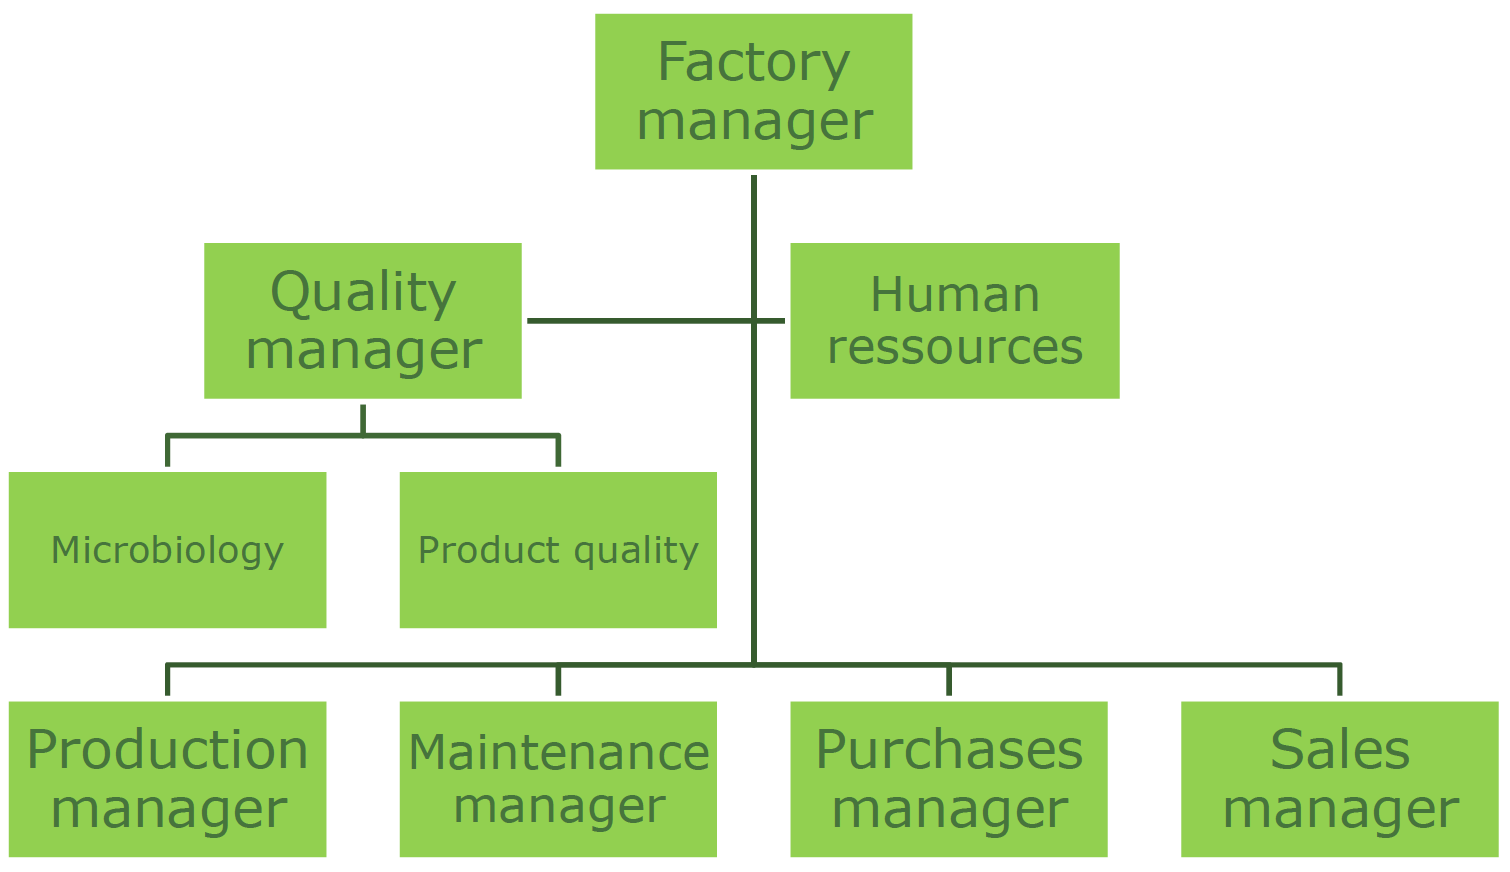
\includegraphics[width=0.8\textwidth]{Figures/Parma Ham - Organization Diagram.png}
    \caption{Organizational structure of Parma Ham A/S}
    \label{fig:ParmaHamAS}
\end{figure}

\subsubsection*{Responsibilities}
 
\begin{highlight}
    The information given for the organizational structure and roles is as follows:

\begin{itemize}
\item The Factory Manager is responsible for:
\subitem - The overall management of the factory, including the implementation of 
\subitem - The FSMS.
\subitem - Shall ensure adequate ressources for development and implementation of the Food Safety \subitem Management System and for continually improving its effectiveness

\item The Quality Manager is the overall responsible for:
\subitem - The Food Safety Management System
\subsubitem * Development
\subsubitem * Implementation
\subsubitem * Maintenance

\item The Production Manager is responsible for:
\subitem  - The production of the Parma ham and for inspection of raw materials
\subitem - The production staff is divided into
several sections, each with a section leaders
\subitem - The section leaders are responsible for
\subitem - Ensuring that all staff members have the necessary competencies
\subitem - Ensuring that all staff members
have the necessary food safety awareness
\subitem - Education and training of staff members

\end{itemize}
\end{highlight}

\begin{highlight}
    Information continued:
    \begin{itemize}
        \item The Sales Manager is responsible for:
        \subitem - Customer focus
        \subitem - Investigating the requirements and expectations of customers
        \subitem - Investigating whether these requirements and expectations are fulfilled

        \item The Purchasing Manager is responsible for:
        \subitem - Supplier focus
        \subitem - Ensuring that purchased products conform to specified purchase requirements
        \subitem - Specified purchase requirements
        \subsubitem * Approval of products, procedures, processes and equipment
        \subsubitem * Qualification of personnel
        \subsubitem * QMS/FSMS
        \subitem - Supplier audits

    \end{itemize}
\end{highlight}


